\future{\improve{Write an introduction}}

\section{2-Bundles}

\begin{definition}
 A \define{$2$-bundle} consists of 2-spaces $E$ and $B$ together with a smooth map $p:E\rightarrow B$.
\end{definition}
To consider \emph{locally trivial} 2-bundles, we would need to categorify the concept of open cover to obtain a ``2-cover'' of the base 2-space $B$. However this isn't easy and isn't required for the main 2-bundles we will later study, so for us $B$ is an ordinary smooth space (or a smooth 2-space with only identity morphisms).
Note in the following that by Property (\ref{restrict}) one can restrict a 2-bundle $p:E\rightarrow B$ to $p:E_{|U}\rightarrow B$ to any subspace $U\subset B$.
\begin{definition}
 Let $F$ be a smooth 2-space. A \define{locally trivial 2-bundle with fibre F} is a 2-bundle $p:E\rightarrow B$ together with an open cover $\{U_i\}$ of $B$ and smooth equivalences $\xymatrix{E_{|U_i}\ar[r]^{t_i} & U_i\times F}$ such that the diagrams
\begin{equation}    \label{commute2}
 \xymatrix{E_{|U_i}\ar[rr]^{t_i} \ar[dr]^{p} & & U_i\times F \ar[dl]\\
& U_i & }
\end{equation}

commute. We call the $t_i$'s the \define{local trivializations}.
\end{definition}

By definition of smooth equivalence, this means we have smooth maps \[ \bar{t_i}:U_i\times F\rightarrow E_{|U_i}                                                                \]
together with invertible 2-maps \begin{align*}
                                 \sigma_i : t_i\bar{t}_i &\Rightarrow 1_{E_{|U_i}}\\
				\bar{\sigma}_i: \bar{t}_i t_i &\Rightarrow 1_{U_i\times F}
                                \end{align*}
Over the intersection $U_{ij}$, we get an autoequivalence \[ \bar{t}_i t_j:U_{ij}\times F\rightarrow U_{ij}\times F
                                                          \]
which by diagram (\ref{commute2}), acts trivially on $U_{ij}$ and

\[ \bar{t}_i t_j(x,f)=(x,fg_{ij}(x))
\]
for some smooth map $g_{ij}$ from $U_{ij}$ to the smooth space of autoequivalences of $F$, the \define{transition functions}. As we previously saw this corresponds to a map \[ g_{ij}:U_{ij}\rightarrow \mathcal{AUT}(F)_0
	\]
Note that $\mathcal{AUT}(F)$ has a structure of a \emph{weak} 2-group (as mentioned in the introduction), with the operation of composition.

Let us consider the triple intersection $U_{ijk}$. Composing horizontally we get the invertible 2-map
\[
 \bar{t}_i\sigma_j t_k:\bar{t}_i  t_j\bar{t}_j t_k \Rightarrow \bar{t}_i t_k 
\]

But \begin{align*} 
         \bar{t}_i t_j \bar{t}_j t_k(x,f)&=(x,fg_{ij}(x)g_{jk}(x)),\\
         \bar{t}_i t_k  (x,f)&=(x,fg_{ik}(x))
    \end{align*}
 \[
      \therefore \qquad \bar{t}_i \sigma_j t_k(x,f):(x,fg_{ij}(x)g_{jk}(x))\rightarrow (x,fg_{ik}(x))
   \]

This morphism is the identity on $x$ and so it must be of the form\[ \bar{t}_i\sigma_j t_k(x,f)=(1_x,fh_{ijk}(x))\]
for some map \index{$h_{ijk}$} $h_{ijk}(x):g_{ij}(x)g_{jk}(x)\rightarrow g_{ik}(x)$ depending smoothly on $x$. Similarly taking $U_{ii}$ one obtains smooth maps \[k_i:U_i\rightarrow (\mathcal{AUT}(F))_1
\]
such that for any $x\in U_i$, \index{$k_i$} $k_i(x):g_{ii}(x)\rightarrow 1_{\mathcal{AUT}(F)}$.
We have obtained a categorification of the cocycle condition in bundles, where now $g_{ik}=g_{ij}g_{jk}$ holds only up to the isomorphisms $h_{ijk},k_{i}$, the \define{higher transition functions}.

%% Note that, by the interchange law (\ref{interchangelaw}), 
%% 
%% \begin{align*}
%% (\sigma_j \circ (t_k\circ \bar{t_k}))\bullet (1_{E_{|U_i}}\circ \sigma_k)&=(\sigma_j \bullet 1_{E_{|U_i}} )\circ ((t_k\circ \bar{t}_k)\bullet \sigma_k)\\
%% &= \sigma_j \circ ((t_k\circ \bar{t}_k)\bullet \sigma_k)
%% \end{align*}
%% 
%% Thus, composing horizontally with $(t_i\bullet \bar{t}_i)$ and repeatedly applying the interchange law:
%% 
%% \begin{align*}
%% (t_i\bullet \bar{t}_i) \circ ((\sigma_j \circ (t_k\circ \bar{t}_k))\bullet (1_{E_{|U_i}}\circ \sigma_k))&=(t_i\bullet \bar{t}_i) \circ ((\sigma_j \bullet 1_{E_{|U_i}} )\circ ((t_k\circ \bar{t}_k)\bullet \sigma_k))\\
%% \Leftrightarrow (t_i \circ (\sigma_j \circ (t_k\circ \bar{t}_k)))\bullet (\bar{t}_i \circ (1_{E_{|U_i}}\circ \sigma_k)) &= (t_i\circ (\sigma_j \bullet 1_{E_{|U_i}} ))\bullet (\bar{t}_i \circ ((t_k\circ \bar{t}_k)\bullet \sigma_k)))
%% \end{align*} 

\begin{prop}
\begin{equation}\label{cococycle} (h_{ijk}\circ g_{kl})\bullet h_{ikl} = (g_{ij}\circ h_{jkl})\bullet h_{ijl}\end{equation} 
\end{prop}
\begin{proof}
In fact, we prove that
\[ ((\bar{t}_i\circ\sigma_j \circ t_k)\circ \bar{t}_k\circ t_l)\bullet (\bar{t}_i\circ \sigma_k\circ t_l) = ((\bar{t}_i\circ t_j) \circ (\bar{t}_j\circ \sigma_k\circ t_l))\bullet ((t_i\circ \sigma_j)\circ t_l)
\]

This is achieved by repeated iterations of the interchange law (\ref{interchangelaw}). On one hand,
\begin{align*}
((\bar{t}_i\circ\sigma_j \circ t_k)\circ \bar{t}_k\circ t_l)\bullet (\bar{t}_i\circ \sigma_k\circ t_l)&=(\bar{t}_i\bullet \bar{t}_i)\circ ((\sigma_j\circ t_k\circ\bar{t}_k\circ t_l)\bullet (\sigma_k\circ t_l))\\
&= \bar{t}_i\circ ((\sigma_j \circ t_k \circ \bar{t})\bullet \sigma_k )\circ (t_l\bullet t_l)\\
&= \bar{t_i}\circ ((\sigma_j\circ t_k\circ \bar{t}_k)\bullet (1_{E_{|U_j}}\circ \sigma_k))\circ t_l\\
&= \bar{t_i}\circ (\sigma_j\bullet 1_{E_{|U_j}})\circ ((t_k\circ \bar{t}_k)\circ \sigma_k)  \circ t_l\\
&= \bar{t_i}\circ \sigma_j \circ \sigma_k \circ t_l
\end{align*}

On the other hand,
\begin{align*}
((\bar{t}_i\circ t_j) \circ (\bar{t}_j\circ \sigma_k\circ t_l))\bullet ((t_i\circ \sigma_j)\circ t_l) &= ((\bar{t}_i\circ t_j\circ \bar{t}_j\circ \sigma_k)\bullet (\bar{t}_i\circ \sigma_j))\circ (t_l\bullet t_l)\\
&= ((\bar{t}_i\bullet \bar{t}_i)\circ ((t_j\circ \bar{t}_j \circ \sigma_j )\bullet \sigma_j )\circ t_l\\
&= \bar{t}_i \circ ((t_j\circ \bar{t}_j\circ \sigma_k)\bullet (\sigma_j \circ 1_{E_{|U_k}}))\circ t_l \\
&= \bar{t}_i \circ (((t_j\circ \bar{t}_j)\bullet \sigma_j)\circ (\sigma_k \bullet 1_{E_{|U_k}} ))\circ t_l \\
&= \bar{t}_i \circ \sigma_j \circ \sigma_k \circ t_l 
\end{align*}
\end{proof}


That is, the following diagram (the \define{associative law}) commutes:

% Note that, by definition, these isomorphisms make the following diagram (the \define{associative law} and the \define{left and right unit laws}) commute:

\[
 \xymatrix{& g_{ij}(x)g_{jk}(x)g_{kl}(x)\ar[dl]^{h_{ijk}(x)g_{kl}(x)} \ar[dr]^{g_{ij}(x)h_{jkl}(x)} &\\
g_{ik}(x)g_{kl}(x)\ar[dr]^{h_{ikl}(x)}& & g_{ij}(x)g_{jl}(x)\ar[dl]^{h_{ijl}(x)}\\
& g_{il}(x) &}
\]

% \[
%  \xymatrix{ g_{ii}(x)g_{ij}(x)\ar[rr]^{k_i(x)g_{ij}(x)} \ar[drr]^{h_{iij}(x)} & &  g_{ij}(x) \ar[d]^{h_{iij}(x)}   \\
%  &  & g_{ij}(x)}  
%  \qquad \xymatrix{ g_{ij}(x)1 \ar[d]^{=} & & g_{ij}(x)g_{jj}(x) \ar[ll]^{g_{ij}(x)k_j(x)} \ar[dll]^{h_{ijj}(x)} \\
% g_{ij}(x) &  &}
% \]

%\improve{Final version will have more here...}

This can best be understood in terms of the tetrahedral diagram:
\begin{eqnarray*}
\begin{picture}(140,160)
  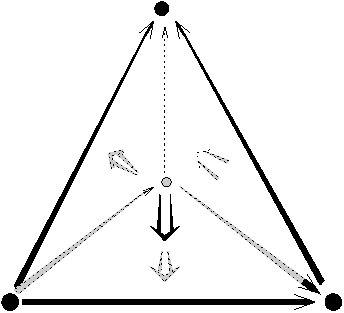
\includegraphics{figures/tetrahedron}
  \put(-127,46){${}_{g_{ij}}$}
  \put(-53,46){${}_{g_{jk}}$}
  \put(-90,-3){$g_{ik}$}
  \put(-137,80){$g_{il}$}
  \put(-41,80){$g_{kl}$}
  \put(-82,105){${}_{g_{jl}}$}

  \put(-80,22){$h_{ijk}$}
  \put(-82,47){$h_{ikl}$}
  \put(-68,85){${}_{h_{jkl}}$}
  \put(-112,85){${}_{h_{ijl}}$}
\end{picture}
\end{eqnarray*}

% \begin{displaymath}
%  \xymatrix@+4pc{
% & \bullet & \\
% & \ar@*{[|(20)]}[dr]^{g_{jk}} \ar[u]^{g_{jl}} & \\
% \ar[rr]_{g_{ik}} \ar[uur]^{g_{il}} \ar[ur]^{g_{ij}} & & \ar[uul]^{g_{kl}} \\}
% \end{displaymath}



\begin{definition}\label{g2bundle}
Let $\mathcal{G}$ be a smooth 2-group, and $\mathcal{F}$ a smooth space. A (strict) \define{action} of $\mathcal{G}$ in $\mathcal{F}$ is a smooth map \[
                        \alpha:\mathcal{G}\rightarrow \mathcal{AUT}(\mathcal{F})
                       \]
that preserves products and inverses (i.e., a \define{smooth homomorphism}).
We say that a locally trivial 2-bundle has \define{structure 2-group} $\mathcal{G}$, when $g,h$ and $k$ (defined above) factor through an action $\mathcal{G}\rightarrow\mathcal{AUT}(\mathcal{F})$. In this case, $E$ is said to be a \define{$\mathcal{G}$-2-bundle}. Furthermore, when $\mathcal{F}=\mathcal{G}$ it is said to be a  \define{principal $\mathcal{G}$-2-bundle}.
\end{definition}




\section{2-Bundles with 2-Connections}
%\improve{final version will change here, starting with diagrams which were temporarily borrowed}

In order to categorify the notion of holonomy we need the following description of a connection in terms of local holonomy functors from \cite{baez-2004}:

\begin{theorem}
Let $(E,p,B)$ be a principal $G$-bundle of smooth spaces with a smooth structure group, locally trivialized over a cover $\{ U_i\}_{i\in I}$ with corresponding transition functions $g_{ij}$. There is a bijection between connections on $E$ and smooth maps of 2-spaces \[
hol_i:P^1_1(U_i)\rightarrow G
\]
for each $i\in I$, such that:
each $g_{ij}$ defines a smooth natural isomorphism $hol_{i|U_{ij}}\rightarrow hol_{j|U_{ij}}$.
\end{theorem}

%% Recall that a connection assigned an element of the structure group to paths in the base space. We then expect a 2-connection to assign to each path an object of the structure 2-group, and to each ``surface'' a morphism. By ``surface'' we mean the following:

That is, the diagram below commutes, for every path $\gamma$ in $U_{ij}$ connecting $x$ and $y$.

\[
\xymatrix{\bullet \ar[rr]^{g_{ij}(x)} \ar[dd]_{hol_i(\gamma)} & & \bullet \ar[dd]^{hol_j(\gamma)}\\
\\
\bullet \ar[rr]_{g_{ij}(y)} & & \bullet
}
\]

And from the cocycle equation $g_{ik}=g_{ij}g_{jk}$,
\[
\xymatrix{ & hol_j \ar[ddr]^{g_{jk}} &\\
\\
hol_i \ar[uur]^{g_{ij}} \ar[rr]_{g_{ik}} & & hol_k}
\]

\begin{definition}
 Let $M$ be a smooth space. A \define{parametrized bigon} in $M$ is a smooth map\[
                                                                                 \Sigma:[0,1]\times [0,1]\rightarrow M
                                                                                \]
where $\Sigma(s,\cdotp)$ is constant for $s$ in a neighborhood of 0 and 1, and $\Sigma(s,t)$ is independent of $t$ when $t$ approaches 0 and 1. $\gamma_0=\Sigma(\cdotp,0)$ and $\gamma_1=\Sigma(\cdotp,1)$ are said to be the \define{source} and \define{target} of $\Sigma$ respectively. We write $\Sigma:\gamma_0\rightarrow \gamma_1$.
We generalize the notion of path groupoid again using the notion of thin homotopy.
\end{definition}
\begin{definition}
 Let $M$ be a smooth space, and $\Sigma:\gamma_0\rightarrow \gamma_1$ and $\Sigma':\gamma_0'\rightarrow \gamma_1'$ be parametrized bigons in $M$. A \define{thin homotopy} between $\Sigma$ and $\Sigma'$ is a smooth map $H:[0,1]^3\rightarrow M$ such that
\begin{itemize}
 \item $\text{rank}(dH(s,t,u))< 3$ for all $s,t,u$.
 \item $H(s,t,0)=\Sigma(s,t)$,
 \item $H(s,t,1)=\Sigma'(s,t)$,
\item $H(s,t,u)$ is independent of $u$ in a neighborhood of $u=0$ and 1, and it is constant near $s=0$ and 1,
\item for $t$ in a neighborhood of 0 we have that $H(s,t,u)=H_0(s,u)$ for some thin homotopy from $\gamma_0$ and $\gamma_0'$,
\item for $t$ in a neighborhood of 1 we have that $H(s,t,u)=H_1(s,u)$ for some thin homotopy from $\gamma_1$ and $\gamma_1'$,
\end{itemize}
As before this forms an equivalence relation, and two parametrized bigons $\Sigma,\Sigma'$ are said to have the same thin homotopy class if they are thinly homotopic. To a class of this relation we call a \define{bigon}, the class above being written $[\Sigma]$.
The \define{path 2-groupoid} $P_2(B)$ of a smooth space $B$ is the 2-category whose objects are the points of $B$, morphisms are thin homotopy classes of paths $[\gamma]$ in $B$ that are constant near the edges, and 2-morphisms are bigons in $B$, represented by (taking $x=\gamma(0)$, $y=\gamma(1)$)
\[
 \xymatrix{ x \ar@/^1pc/[rr]^{[\gamma_0]}_{}="0"
           \ar@/_1pc/[rr]_{[\gamma_1]}="1"
           \ar@{=>}"0";"1"^{[\Sigma]} && y}
\]
with the natural compositions (see \cite{baez-2004}).
\end{definition}

It is left to check that this has a structure of a smooth 2-category. Here we are implicitly stating the internalization process defined in the beginning has a straightforward generalization, so that a smooth 2-category is a 2-category internalized in $C^\infty$.

\begin{definition}
 Let $p:E\rightarrow B$ be a $\mathcal{G}$-2-bundle as in Definition \ref{g2bundle}, where for simplicity we assume that $k_i=1$. A \define{2-connection} is a tuple of the following:
%\improve{duvida}
\begin{itemize}
 \item Smooth 2-functors $hol_i:P_2(U_i)\rightarrow \mathcal{G}$,
\item Pseudonatural isomorphisms \[
                           g_{ij}:hol_i|_{P(U_{ij})}\rightarrow hol_j|_{P(U_{ij})}
                          \]
extending the transition functions. That is, for each $\gamma:x\rightarrow y$ in $U_{ij}$ a morphism

\begin{center}
\begin{picture}(100,100)
  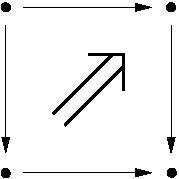
\includegraphics{figures/filled_square}
  \put(-60,90){$g_{ij}\of{x}$}
  \put(-60,-8){$g_{ij}\of{y}$}
  \put(-120,42){$\hol_i(\gamma)$}
  \put(0,42){$\hol_j(\gamma)$}
  \put(-75,50){$g_{ij}\of{\gamma}$}
\end{picture}
\vskip 0.5em
\end{center}
depending smoothly on the path $\gamma$, that makes the following diagram commute:\\
\begin{eqnarray*}
\begin{picture}(240,140)
 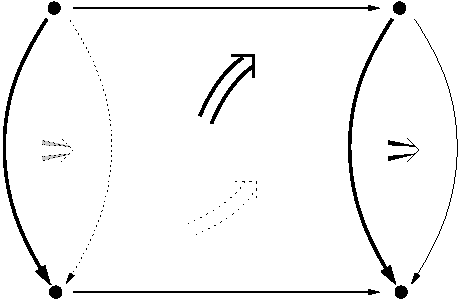
\includegraphics{figures/tincan}
 \put(-3,-17){	
 \begin{picture}(0,0)
 \put(122,0){
  \begin{picture}(0,0)
   \put(-385,90){$\hol_i\of{\gamma}$}
   \put(-290,100){${}_{\hol_i\of{\eta}}$}
   \put(-333,100){$\hol_i\of{\Sigma}$}
   \put(-242,50){${}_{g_{ij}\of{\eta}}$}
   \put(-268,125){${g_{ij}\of{\gamma}}$}
   \put(-250,163){$g_{ij}\of{x}$}
   \put(-250,10){$g_{ij}\of{y}$}
  \end{picture}}
 \put(288,0){
  \begin{picture}(0,0)
   \put(-382,90){$\hol_j\of{\gamma}$}
   \put(-290,100){${}_{\hol_j\of{\eta}}$}
   \put(-333,100){$\hol_j\of{\Sigma}$}
  \end{picture}}
 \end{picture}}
\end{picture}
\end{eqnarray*}
for any bigon $\Sigma: \gamma \Rightarrow \eta$ in $U_{ij}$,
\item modifications $h_{ijk}$ (induced by the transition functions $h_{ijk}$):
\[
 \xymatrix{& hol_j \ar[ddr]^{g_{jk}} \ar@{=>}[dd]^{h_{ijk}} &\\
\\
hol_i \ar[uur]^{g_{ij}} \ar[rr]_{g_{ik}} & & hol_k}
\]

That is, the following commutes:

\begin{center}
\begin{picture}(180,270)
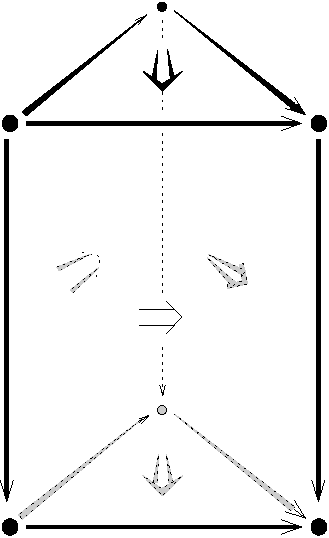
\includegraphics{figures/prism}
  \put(-3,100){$\hol_k\of{\gamma}$}
  \put(-190,100){$\hol_i\of{\gamma}$}
  \put(-80,160){${}_{\hol_j\of{\gamma}}$}
  \put(-100,-7){$g_{ik}\of{y}$}
  \put(-100,187){$g_{ik}\of{x}$}
  \put(-138,43){${}_{g_{ij}\of{y}}$}
  \put(-138,237){${}_{g_{ij}\of{x}}$}
  \put(-47,43){${}_{g_{jk}\of{y}}$}
  \put(-47,237){${}_{g_{jk}\of{x}}$}
  \put(-95,16){${}_{h_{ijk}\of{y}}$}
  \put(-95,212){${}_{h_{ijk}\of{x}}$}
  \put(-100,90){$g_{ik}\of{\gamma}$}
  \put(-150,124){${}_{g_{ij}\of{\gamma}}$}
  \put(-50,117){${}_{g_{jk}\of{\gamma}}$}
\end{picture}
\end{center}
for any bigon $\Sigma : \gamma \Rightarrow \eta$ in $U_{ijk}$.
\end{itemize}

\end{definition}

The following is one of the main results in \cite{baez-2004}.

\begin{theorem}
 Let $p:E\rightarrow B$ be a principal $\mathcal{G}$-2-bundle, locally trivial over an open cover $\{U_i\}$. Suppose that $k_i=1$. Let $(G,H,\partial,\vartriangleright)$ be the Lie crossed module associated to $\mathcal{G}$, with differential Lie crossed module $(\mathfrak{g},\mathfrak{h},\partial,\vartriangleright)$.

Then there is a one-to-one correspondence between 2-connections on $E$ and differential forms $(A_i,B_i,a_{ij})\in \Omega^1(U_i,\mathfrak{g})\times \Omega^2(U_i,\mathfrak{h})\times \Omega^1(U_{ij},\mathfrak{h})$ such that:
\begin{enumerate}
 \item \label{fakec} $F_{A_i}+\partial(B_i)=0$, where $F_{A_i}=dA_i+A_i\wedge A_i$ (the \define{curvature 2-form} of $A_i$).
\item $A_i=g_{ij}A_jg_{ij}^{-1}+g_{ij}dg_{ij}^{-1}-\partial (a_{ij})$
\item $B_i=g_{ij}\vartriangleright B_j+k_{ij}$ where $k_{ij}=da_{ij}+a_{ij}\wedge a_{ij}+d\alpha (A_i)\wedge a_{ij}$
\item $a_{ij}+g_{ij}\vartriangleright a_{jk}=h_{ijk}a_{ik}h_{ijk}^{-1}+(dh_{ijk})h_{ijk}^{-1}+(A_i\vartriangleright h_{ijk})h_{ijk}^{-1}$
\end{enumerate}
\end{theorem}

\future{\improve{ver relacao disto com o teorema do Picken para bundles com conexao. la o grupo de estrutura codificava o fibrado? e era a holonomia que dava a conexao. aqui fixamos o grupo...}}


\subsection{Gerbes}
%\improve{This section will be more developed in the final version}
\future{\improve{construcao toda no 2-bundles do bartels, pag. 74}}
This reduces to the case of \define{abelian gerbes}  with connections when $k_i=1$ and $F=\mathcal{G}$ is as in Example \ref{abgerb}. Similarly we arrive at \define{nonabelian gerbes} when $k_i=1$ and $F=\mathcal{G}$ is as in Example \ref{nabgerb}. Recall that equivalence classes of gerbes correspond bijectively to the elements in $\check{H}^2(M,\underline{S^1}_B)$ (see \cite[p. 10]{picken_parallel}).

\future{In \cite{bartels-2004} the 2-category of $\mathcal{G}$-2-bundles is defined and shown to be equivalent to the 2-category of abelian or nonabelian gerbes, when $\mathcal{G}$ is as above.
\improve{ver todas as condicoes. por exemplo, so englobam os gerbes com fake curvature (as introduced in \cite{breen-2001}), by condition (\ref{fakec})}.
 \improve{falar de fake curvature, de onde vem - Breen Messing}}

\newpage
\section{Categorical connections} \label{catconn}
We now focus on a particular kind of 2-connection introduced in \cite{picken_faria} by Martins and Picken, which can be used to define parallel transport. Here we address the question of the existence of such connections.

% Our construction corresponds to the particular case of $\mathcal{G}$-2-bundles introduced in \cite{picken_faria}, for which the $E$ valued transition functions are trivial, and therefore the $G-$valued transition functions satisfy the usual cocycle condition for a principal $G$-bundle. More specifically we will study a particular 2-connection in certain 2-bundles, as we hope to make clear later.

\begin{definition}
 Let $\mathcal{G}=(\partial :H\rightarrow G,\vartriangleright)$ be a crossed module, with associated differential crossed module $\mathfrak{G}=(\partial:\mathfrak{h}\rightarrow \mathfrak{g},\vartriangleright)$. A \define{$\mathcal{G}$-categorical connection} on a principal $G$-bundle $p:E \rightarrow B$ is a pair $(m,\omega)$ where $\omega\in \Omega^1(E,\mathfrak{g})$ is a connection 1-form on $E$ and $m$ is an equivariant horizontal 2-form in $\Omega^2(E,\mathfrak{h})$, such that
\begin{equation}
\partial (m)=\Omega \label{vanish}
\end{equation}
\end{definition}
By saying that $m$ is equivariant we mean that for all $g\in G$, $(R_g)^*m=g^{-1} \vartriangleright m$. It should be remarked that condition (\ref{vanish}) corresponds to the \emph{vanishing of the fake curvature} as introduced in \cite{breen-2001}.

\begin{definition}
 To a categorical connection as above, we associate the \define{2-curvature} 3-form as
\[
 \mathcal{M}=dm(H\times H\times H)
\]
\end{definition}


\begin{definition}\label{rw}
 Let $\omega \in \Omega^n(M,\mathfrak{g})$ and $\eta\in \Omega^m(M,\mathfrak{h})$. We define the \define{covariant tensor field} on $M$ with values in $\mathfrak{h}$ is defined by
\[
 (\omega\otimes^\vartriangleright \eta)(A_1,\ldots,A_n,B_1,\ldots,B_m)=\omega(A_1,\ldots,A_n)\vartriangleright \eta(B_1,\ldots,B_m), \quad A_i,B_i\in \mathfrak{X}(M)
\]
This gives us a natural \define{alternating tensor field} $\omega\wedge^\vartriangleright \eta \in \Omega^{n+m}(M,\mathfrak{h})$ with
\[
 \omega\wedge^\vartriangleright \eta=\frac{(n+m)!}{n!m!}\text{Alt}(\omega\otimes^\vartriangleright\eta)
\]
\end{definition}

\begin{example}
Let $\mathcal{G}=(\text{id}:G\rightarrow G,\vartriangleright)$, where $\vartriangleright$ is the adjoint action of $G$ on $G$.

Let $p:E\rightarrow B$ be principal $G$-bundle with connection one-form $\omega$. Then $(\omega,m)$ is a $\mathcal{G}$-categorical connection, where $m=\Omega$ is the curvature 2-form of $\omega$.

Note that in terms of Definition \ref{rw} the \define{structure equation} for the curvature form is
\[
 \Omega=d\omega +\frac{1}{2}\omega\wedge^{\text{ad}}\omega
\]
and the \define{Bianchi identity} is \[
                                          d\Omega+\omega\wedge^{\text{ad}}\Omega=0
                                         \]

\end{example}

\future{\improve{acima nao queria outro ``define'', mas um comando que voltasse a indexar o mesmo nome na mesma entrada}}

\begin{lemma}
 If $\varphi$ is a $G$-equivariant horizontal $(n-1)$-form in $P$, then
\[
 D\varphi =d\varphi +\omega \wedge^{\text{ad}}\varphi
\]

\end{lemma}


\begin{prop}[\index{2-structure equation}2-structure equation]
 \[\mathcal{M}=dm+\omega\wedge^{\vartriangleright}m \]
In particular $\mathcal{M}$ is $G$-equivariant.
\end{prop}

See \cite[p. 79]{kobayashi1} and \cite[p. 19]{picken_faria}.

% This follows partly from the following:
% 
% \begin{lemma}
%  If $\eta\in \Omega^{n-1}(E,\mathfrak{g})$ is $G$-equivariant, then $D\eta=d\eta+\omega\wedge^\vartriangleright \eta$.
% \end{lemma}
% 
% \improve{prove this later (?)}

\begin{prop}[\index{2-Bianchi identity}2-Bianchi identity]
 \[
  d\mathcal{M}(H\times H\times H\times H)=0
 \]
or by the previous lemma,
\[
 d\mathcal{M}+\omega\wedge^\vartriangleright \mathcal{M}=0.
\]
\end{prop}

\subsection{Local forms of the categorical connection}
Take an open cover $\{U_\alpha\}_\alpha$ of $B$ that trivializes our bundle. Taking local sections $f_\alpha:U_\alpha\rightarrow E_\alpha$, the local forms are given by \[
              m_\alpha=(f_\alpha)^*m
		   \]
\[
 \omega_\alpha=(f_\alpha)^*\omega
\]

We have already characterized the local form of $\omega$ and $\Omega$. Note that, defining  $\phi_{\alpha,\beta}:U_{\alpha,\beta}\rightarrow G$ by $f_\alpha (x)\phi_{\alpha,\beta}(x)=f_\beta(x)$,  from the $G$-invariance of $m$ and $\mathcal{M}$ we get:

\[
 m_\beta(X,Y)=\phi_{\alpha,\beta}^{-1}\vartriangleright m_\alpha(X,Y)
\]
\[
 \mathcal{M}_\beta (X,Y,Z)=\phi_{\alpha,\beta}^{-1}\vartriangleright \mathcal{M}_\alpha(X,Y,Z)
\]
for each $X,Y\in \mathfrak{X}(U_{\alpha\beta})$.


\begin{prop}\label{localform}
 Let $H,G$ be Lie groups, $B$ a smooth manifold and $E\rightarrow B$ a principal $G$-bundle. Let $\mathscr{G}=(\partial:H\rightarrow G,\vartriangleright)$ be a Lie crossed module and $\mathfrak{G}=(\partial:\mathfrak{h}\rightarrow\mathfrak{g},\triangleright)$ its associated differential crossed module.
Then a pair $(\omega,m)\in \Omega^2(E,\mathfrak{g})\times \Omega^1(E,\mathfrak{h})$ is a $\mathscr{G}-$categorical connection on $E$ if and only if there are local sections $f_\alpha:U_\alpha\rightarrow E_\alpha$ of $E$ (where $\{U_\alpha\}_\alpha$ is an open cover of $B$) and local forms $(\omega_\alpha,m_\alpha)\in \Omega^1(U_\alpha,\mathfrak{g})\times\Omega^2(U_\alpha,\mathfrak{h})$ with the following properties for each $U_{\alpha\beta}\neq\emptyset$: defining $\phi_{\alpha,\beta}:U_{\alpha,\beta}\rightarrow G$ by $f_\alpha (x)\phi_{\alpha,\beta}(x)=f_\beta(x)$, 

\begin{align}
 \partial(m_\alpha)&=\Omega_\alpha=d\omega_\alpha+\frac{1}{2}\omega_\alpha\wedge^{ad} \omega_\alpha \label{partialomega} \\
 \omega_\beta(X)&=\phi^{-1}_{\alpha,\beta}\omega_\alpha(X)\phi_{\alpha,\beta}+\phi^{-1}_{\alpha,\beta}d\phi_{\alpha,\beta} \label{connection}\\
 m_\beta(X,Y)&=\phi^{-1}_{\alpha,\beta}\triangleright m_\alpha(X,Y) \label{compatform}
\end{align}
for each $X,Y\in \mathfrak{X}(B)$.
\end{prop}
\begin{lemma}
Let $(E,p,B)$ be the trivial bundle $E=B\times G$. Given $(\omega_0,m_0)\in \Omega^1(B,\mathfrak{g})\times \Omega^2(B,\mathfrak{h})$ such that $\partial(m_0)=\Omega_0$, there exists a $\mathcal{G}$-categorical form $(\omega,m)$ with local forms $(\omega_0,m_0)$.
\end{lemma}
\begin{proof}

Let $\theta$ be the canonical left invariant $\mathfrak{g}$-valued form on $G$ (see Equation (\ref{maurercartan})). Let $f:B\rightarrow E$ be the trivial section $f(x)=(x,e)$ (where $e$ is the identity of $G$). Then $\omega_{(x,g)}=g^{-1}p^*(\omega_0)g+\theta$ is a connection 1-form on $E=M\times G$ with local form $\omega_0$ (this is a classical construction, see \cite[p. 67]{kobayashi1}).
Define $m$ for any $(x,g)\in B\times G$ and $X,Y\in T_{(x,g)}E$ by \[
m(X,Y)=g^{-1}\vartriangleright p^*(m_0)(X,Y)
\]
This 2-form is horizontal since clearly $p^*(m_0)$ is horizontal. For $G$-invariance, let $X,Y\in T_{(x,g)}E$.
\begin{align*}
 (R_h^*m)_g(X,Y)&=m_{gh}(Xh,Yh)\\
&=(gh)^{-1}\vartriangleright p^*(m_0)(Xh,Yh)\\
&=h^{-1}g^{-1}\vartriangleright p^*(m_0)(X,Y)\\
&=h^{-1}\vartriangleright m(X,Y)
\end{align*}

Also recall that $\Omega(X,Y)=g^{-1}p^*(\Omega_0)(X,Y)g$, therefore:
\begin{align*}
\partial (m) (X,Y)&= \partial(g^{-1}\vartriangleright p^*(m_0)(X,Y))\\
& =g^{-1}\partial (p^*(m_0)(X,Y)) g\\
& =g^{-1}p^*(\partial(m_0))(X,Y) g\\
& =g^{-1}p^*(\Omega_0)(X,Y)g\\
& =\Omega(X,Y)
\end{align*}

\end{proof}

%  \notsute{is an cover  $\{U_\alpha\}$ of $M$ such that $E_\alpha=E|U_\alpha$ is trivial}, and local sections $f_\alpha:U_\alpha\rightarrow E_\alpha$ of $P$ (defining $\phi_{\alpha,\beta}:U_{\alpha,\beta}\rightarrow G$ by $f_\alpha (x)\phi_{\alpha,\beta}(x)=f_\beta(x)$
% 
% $(\omega_\alpha,m_\alpha)\in \Omega^1(U_\alpha,\mathfrak{g})\times\Omega^2(U_\alpha,\mathfrak{e})$ 
% 	
%  such that for $U_{\alpha,\beta}\neq\emptyset$:
% \begin{align*}
%  \partial(m_\alpha)&=\Omega_\alpha=d\omega_\alpha+\frac{1}{2}\omega_\alpha\wedge^{ad} \omega_\alpha \\
%  \omega_\beta(X)&=\phi^{-1}_{\alpha,\beta}\omega_\alpha(X)\phi_{\alpha,\beta}+\phi^{-1}_{\alpha,\beta}d\phi_{\alpha,\beta}\\
%  m_\beta(X,Y)&=\phi^{-1}_{\alpha,\beta}\triangleright m_\alpha(X,Y)
% \end{align*}


\subsection{Existence}\label{existence}
A connection 1-form on any bundle can always be found by the means of partitions of unity (see for instance \cite[p. 67]{kobayashi1}). Our problem lies with the form $m$. For that, we describe it in the following terms (as in \cite[p. 75]{kobayashi1}).

\begin{definition}\label{tensdef}
Let $(E,p,B)$ be a principal $G$-bundle. Let $(\rho,V)$ be a representation of $G$ in a finite dimensional vector space $V$. A \define{tensorial form} of degree $k$ on $E$ of type $(\rho,V)$ is a form $\varphi\in\Omega^k (E,V)$ such that
\begin{itemize}
\item $\varphi$ is $G$-invariant for the induced action of $G$ on $V$, i.e. $R_g^*=\rho(g^{-1})\varphi$,
\item $\varphi$ is horizontal, i.e. $\varphi(X_1,\ldots,X_k)=0$ when one of the tangent vectors $X_i$ is vertical.
\end{itemize}
\end{definition}

\begin{example}\label{tensorialexample}
A connection $\omega$ is a tensorial form of degree 1 in $E$ of type $(\text{Ad},\mathfrak{g})$. By definition, $m$ is a tensorial form of degree 2 in $E$ of type $(\vartriangleright,\mathfrak{h})$.
\end{example}


\begin{lemma}\label{tensorialform}
Let $(E',q,B)$ be the bundle associated with the principal $G$-bundle $(E,p,B)$ with fibre $V$, where $G$ acts naturally by $\rho$. There is a one-to-one correspondence between the tensorial forms as above and sections of the bundle \[
\xymatrix{\wedge^k T^*B\otimes E' \ar[d]\\
B} \]
\end{lemma}

\begin{proof}
The associated bundle with fibre $V$ has total space $E'=E \times V / \sim$ where $(eg,x)\sim (e,gx)$. Then each $u\in E$ defines a linear mapping $V\rightarrow q^{-1}(x)$, where $x=p(u)$ given by $ v\mapsto [(u,v)] $


A tensorial $(\rho,V)$ form of degree $k$ can be regarded as a skew-symmetric multilinear mapping $\widetilde{\varphi}_x: T_x(B)\times \ldots \times T_x(B) \rightarrow q^{-1}(x)$, putting
\[
\widetilde{\varphi}_x(X_1,\ldots,X_k)=u(\varphi(X_1^*,\ldots, X_k^*)), \qquad X_i \in T_x(B)
\]letting $X_i^*$ be any vectors at $u$ such that $p(X_i^*)=X_i$. One verifies that this does not depend on the choice of $u$ or the $X_i^*$'s. Conversely, given $\widetilde{\varphi}_x:T_x(B)\times\ldots\times T_x(B)\rightarrow q^{-1}(x)$ skew-symmetric and multilinear, one obtains a tensorial form of degree $k$ of type $(\rho,V)$ on $E$ defined by
\[
\varphi(X_1^*,\ldots,X_k^*)=u^{-1}(\widetilde{\varphi}_x(p(X_1^*),\ldots,p(X_k^*))), \qquad X_i^*\in T_uE
\]
\end{proof}
\future{\improve{acima escolher melhor a construcao}}


Let \index{$\mathfrak{b}$} $\mathfrak{b}=\text{Ker }\partial$ and fix a connection $\omega$. One immediately notices that for any 2-forms $m, m'\in \Omega^2(E,\mathfrak{h})$ of categorical connections with connection $\omega$, $m-m'$ is in $\Omega^2(E,\mathfrak{b})$. Moreover, given such a 2-form $m$, all others are in $\{m+m_0: m_0\in \Omega^2(E,\mathfrak{b})\}$.
\begin{corollary}
For a connection $\omega$, if the set of forms $m$, such that $(\omega,m)$ is a categorical connection, is non-empty, then it is an affine space over $\Gamma_B(\wedge^2T^*B\otimes \mathfrak{b})$.
\end{corollary}

%% \begin{prop}
%% Let $\xi=(E,p,B)$ be a \notsure{fibre bundle} with connection $\omega$, and let $\mathcal{G}=(\partial:E\rightarrow G)$ a Lie crossed module. The following are equivalent:
%% \begin{enumerate}
%% \item There is a $\mathcal{G}$-categorical connection on $\xi$ with connection $\omega$. \label{1}
%% \item $\text{Im}(\Omega)\subset \mathfrak{a}$, where $\mathfrak{a}=\text{Im }\partial$ \index{$\mathfrak{a}$} \notsure{CHECK, only these??}.\label{2}
%% \item $\xi$ admits a reduction to a structure group $H\subset G$, with Lie algebra $\mathfrak{h}$ contained in $\mathfrak{a}$. \label{3}
%% \end{enumerate}
%% \end{prop}
%% \begin{proof}
%% "Connections always exist".... comment, say below .
%% $(\ref{1})\Rightarrow (\ref{2})$ follows by definition. Suppose $\text{Im}(\Omega)\subset \mathfrak{a}$. By Lemma (\ref{tensorialform})b
%% \end{proof}

\begin{theorem}\label{mainthm}
Let $\xi=(E,p,B)$ be a principal $G$-bundle, and let $\mathcal{G}=(\partial:H\rightarrow G)$ a Lie crossed module. The following are equivalent:
\begin{enumerate}
\item There is a $\mathcal{G}$-categorical connection on $\xi$. \label{1}
\item $\xi$ admits a connection with curvature $2$-form $\Omega$ such that $\text{Im}(\Omega)\subset \mathfrak{a}$, where $\mathfrak{a}=\text{Im }\partial$ \index{$\mathfrak{a}$}.\label{2}
\item $\xi$ admits a reduction to a structure group $G'\subset G$, with Lie algebra $\mathfrak{g}'$ contained in $\mathfrak{a}$. \label{3}
\end{enumerate}
\end{theorem}
\begin{proof}\hspace*{\fill}\\ \begin{itemize}
\item[\footnotesize{$(\ref{1})\Rightarrow (\ref{2})$}] Follows by definition. 
\item[\footnotesize{$(\ref{2})\Rightarrow (\ref{1})$}] Let $(E_1,p_1,B)$ be the associated bundle with fibre $\mathfrak{e}$, and $(E_2,p_2,B)$ with fibre $\mathfrak{a}$. Recall that $E_1=E\times_G \mathfrak{h}$ and $E_2=E\times_G \mathfrak{a}$. $m$ corresponds to a 2-form with values in $E_1$, while $\Omega$ corresponds to a 2-form with values in $E_2$. Since $\partial$ is equivariant, the obvious surjective morphism $\widetilde{\partial}:E_1\rightarrow E_2$ is well defined. 
Now the problem of finding $m$ corresponds to the problem of finding a 2-form with values in $E_1$ that projects to the 2-form corresponding to $\Omega$. But applying Theorem \ref{exactseq} with $\xi=Ker \widetilde{\partial}, \chi=E_1$ and $\eta=E_2$ the projection has a right section $w$, and therefore we can take $m=\omega\circ\Omega$.
\item[\footnotesize{$(\ref{2})\Rightarrow (\ref{3})$}] Let $Hol$ be the holonomy group. By the reduction theorem \ref{redthm}, there is a reduction of the structure group to $Hol$. If $\mathfrak{h}$ denotes its Lie algebra, by Ambrose-Singer (Theorem \ref{ambrosesinger}) and since $\Omega$ is horizontal $\mathfrak{h}=\text{Im } \Omega \subset \mathfrak{a}$.
\item[\footnotesize{$(\ref{3})\Rightarrow (\ref{1})$}] If there is a reduction of the structure group $G$ to $G'$, let $\{U_{\alpha\beta}\}$ be a cover with transition functions $g_{\alpha\beta}$ of $\xi$ with values in $G'$ (which exists by Proposition \ref{redprop}). Denoting the Lie algebra of $Hol$ of the reduced bundle by $\mathfrak{h'}$, we get again by Ambrose-Singer that \[
Im \Omega=\mathfrak{h}'\subset \mathfrak{g}' \subset \mathfrak{a}
\] Then the reduced bundle has a categorical connection (by the equivalence of (1) and (2) proved earlier), and by Proposition \ref{localform} we see that the local categorical connection forms of the cover $\{U_{\alpha\beta}\}$, are also local categorical connection forms on $\xi$.
             \end{itemize}
\end{proof}
It should be noted that the above proof (together with the results used) is constructive.


Alternatively we could have proved $(\ref{3})\Rightarrow (\ref{2})$ by using the fact that the connection in the reduced bundle induces naturally a connection on the bundle by $G$-invariance (it is defined solely by its value in a point in each fibre) together with the main property of the fundamental vector field (see equation \ref{mainproperty}).

\begin{corollary}
 In the conditions of Theorem \ref{mainthm}, if $\partial:\mathfrak{e}\rightarrow \mathfrak{g}$ is surjective there is always a categorical connection on a bundle with structure group $G$.
\end{corollary}

This is the case of the crossed modules in Examples \ref{abgerb} and \ref{trivcross}. Most importantly, a categorical connection doesn't always exist.
\begin{example}
 Let $(H,.)=(\mathbb{R}^n,+)$ and $(G,.)=(GL(n,\mathbb{R}),\circ)$. Take the trivial map $\partial:H\rightarrow G$ together with the action $f\vartriangleright e=f(e)$ of $GL(n,\mathbb{R})$ in $\mathbb{R}^n$. Clearly $\mathcal{G}=(\partial:H\rightarrow G,\vartriangleright)$ is a crossed module. Since $\partial:\mathfrak{h}\rightarrow \mathfrak{g}$ is the zero map, in order for there to be a categorical connection, the holonomy group would have to be a discrete subgroup of $G$. But in general that is not the case: take for instance the frame bundle over $S^2$, with $G=GL(2,\mathbf{R})$ and $H=(\mathbf{R}^2,+)$. If the frame bundle could be reduced to a discrete group then it would be trivial as, for any topological group, principal $G$-bundles over $S^2$ are classified by conjugacy classes in $\pi_1(G)$. In particular there would be a section of the frame bundle and hence a nowhere vanishing tangent vector field to $S^2$ which is impossible by the hairy ball theorem (see Theorem (2.28) in \cite[p. 135]{hatcher}).
\end{example}


\subsubsection{Construction for compact groups}

%% We now try to obtain $\mathscr{G}$-categorical connections on a principal $G$-bundle $E\rightarrow M$, with $E,G$ Lie groups. Notice that a connection one-form $\omega$ of the bundle can always be found with the use of partition functions. Also a choice of local forms $\omega_\alpha\in \Omega(U_\alpha,\mathfrak{g})$ such that (\ref{connection}) is equivalent to a choice of a one-form connection on the bundle. So the problem of finding a $\mathscr{G}$-categorical connection reduces to the problem of finding the 2-form $m$. Let $A=\partial(E)$ and $B=Ker(\partial)\subset E$, with corresponding Lie algebras $\mathfrak{a},\mathfrak{g}$. It is a necessary condition for the existence of a categorical connection that $Im(\Omega)\subset \mathfrak{a}$, so let us assume it is the case. 
In the case where categorical connections exist, we provide an alternative way of getting one when the structure group $G$ is compact.
Notice that a local form $m_\alpha\in \Omega^2(U_\alpha,\mathfrak{e})$ satisfies (\ref{partialomega}) if and only if it is of the form
\[ m_\alpha=r\Omega_\alpha+\varphi_\alpha \]
for a left section $r:\mathfrak{a}\rightarrow \mathfrak{e}$ of $\partial$ (ie, $\partial r=id_\mathfrak{a}$) and a local form $\varphi_\alpha\in\Omega^2(U_\alpha,\mathfrak{b})$.
% for any local trivializations $f_\alpha:U_\alpha\rightarrow E_\alpha$, putting $\omega_\alpha=f^*_\alpha \omega \in \Omega(U_\alpha,\mathfrak{g})$ condition \ref{connection} is automatically satisfied, in fact 
% 
% \improve{ter o $\omega$ e o mesmo que ter os $\omega_\alpha$ com (\ref{connection}) certo?}
We can write (\ref{compatform}) in the form:

\[
 (r\Omega_\beta (X,Y)+\varphi_\beta(X,Y))=\phi_{\alpha,\beta}^{-1}\vartriangleright(r\Omega_\alpha (X,Y))+\phi_{\alpha,\beta}^{-1}\vartriangleright \varphi_\alpha(X,Y)
\]

So it would be sufficient to get
\begin{align}
          r\Omega_\beta(X,Y)&=\phi_{\alpha,\beta}^{-1}\vartriangleright (r\Omega_\alpha)(X,Y) \label{eq} \\
        \varphi_\beta (X,Y)&=\phi_{\alpha,\beta}^{-1}\vartriangleright \varphi_\alpha (X,Y) 
\end{align}

But $\Omega_\beta(X,Y)=\phi_{\alpha,\beta}^{-1}\Omega_\alpha (X,Y)\phi_{\alpha,\beta}=Ad_{\phi_{\alpha,\beta}} \Omega_\alpha(X,Y)$
% for the adjoint action $\circ$:\begin{align*}
%                 G\times \mathfrak{g}&\rightarrow \mathfrak{g}\\
%                (g,v)&\mapsto Ad_g(v)
%                \end{align*}
where $Ad_g$ is the adjoint representation of $G$, the canonical action of $G$ in $\mathfrak{g}$.
\future{\improve{dizer o que e uma representacao}}
% , or the derivative in $e\in G$ of the action $g\in G\mapsto(v\mapsto g^{-1}hg))$.
%with an open cover $\{U_\alpha\}$ such that $P|U_\alpha$ is trivial

So condition (\ref{eq}) is verified when $r$ is $G$-equivariant.

\begin{lemma}
Let $G$ be a compact Lie group acting on $V,W$ linear spaces. Let $T:V\rightarrow W$ be an equivariant linear map. Then there is an equivariant left inverse $R:Im(T)\rightarrow V$ of $T$.
\end{lemma}
\begin{proof}
 Put $A=Im(T)$. One can always find a linear section $R_0$, not necessarily equivariant. In general an equivariant map $f:A\rightarrow V$ is a fixed point of the action $\circ$ given by
\begin{align*}
 G\times Hom(A,V)&\rightarrow Hom(A,V)\\
(g,f)&\mapsto (g\circ f)=(v\mapsto g.f(g^{-1}.v))
\end{align*}
Let $\int (\cdotp) dG$ be the unique (normalized) left-invariant integral on $G$ (see \cite[p. 41]{brocker}).
Define
\begin{align*}
 R:A&\rightarrow V\\
a&\mapsto \int_G\frac{g R_0(g^{-1}a)}{Vol(G)}dg
\end{align*}
It is clearly linear, and by left-invariance of the integral:
\begin{align*}
 (h\circ R)(a)&= hR(h^{-1}a)\\
              &= \int_G \frac{hg R_0((hg)^{-1}a)}{Vol(G)}dg\\
              &= \int_G \frac{g R_0(g^{-1}a)}{Vol(G)}dg\\
	      &= R(a)
\end{align*}

It is also a left inverse since, fixing a base of $V$, $T$ is represented by a matrix $(T_{ij})_{ij}$ and
\begin{align*}
 (T R)(a)&=T\int_G \frac{g R_0(g^{-1}a)}{Vol(G)}dg\\
         &=(T_{ij})_{ij}(\int_G \frac{R_0(g^{-1}a)}{Vol(G)} dg)_{i}\\
         &=(\sum_j T_{ij} \int_G (\frac{R_0(g^{-1}a)}{Vol(G)})_i dg)_i\\
         &=\int_G T(\frac{g R_0(g^{-1}a)}{Vol(G)})dg\\
         &=\int_G \frac{gTR_0(g^{-1}a)}{Vol(G)}dg \\
         &=\int_G \frac{gg^{-1}a}{Vol(G)}dg\\
         &= a
\end{align*}
\end{proof}
With the section given by this proposition, and taking all $\varphi_\alpha$ to be null, we get a connection 2-form $m$ compatible with a given $\omega$ .

\subsubsection{General local construction} Given a categorical connection we will locally construct other categorical connections with the same curvature.  We observed that any two $\mathscr{G}$-categorical connections $(\omega,m)$ and $(\omega,m')$ differ only on an horizontal and equivariant 2-form $\psi=m-m'\in\Omega^2(E,\mathfrak{b})$. There is a correspondence between these forms and the local forms $\psi_\alpha=m_\alpha-m_\alpha'$ (given by $\psi_\alpha=s_\alpha^*\psi$) obeying
\begin{equation}\label{psi}
\psi_\beta=\phi_{\alpha,\beta}^{-1}\vartriangleright \psi_\alpha                                                                                                                                                                                                                                                                                                                                                                                                                                                                                                                                                                               \end{equation}
That is, for a fixed local form  $(\omega_\alpha,m_\alpha)$ of $\mathscr{G}$-categorical connections, any other over the same $\omega$ will be of the form $(\omega_\alpha,m_\alpha+\psi_\alpha)$ for $\psi_\alpha\in\Omega^2(U_\alpha,\mathfrak{b})$ obeying (\ref{psi}).

Since $M$ is second countable it has countable open covers $\{U_i\}_i$ and $\{V_i\}_i$ such that $\bar{V}_i\subset U_i$. Let $m_{i}=s_i^*m$. Then at $U_0$, start with the 2-form $m'_0\in\Omega^2(U_0,\mathfrak{b})$ 
\[
 m_0'=m_{0}+\psi_0
\]
for \emph{any} $\psi_0\in\Omega^2(U_0,\mathfrak{b})$, where $m_0$ is the local form of our initial categorical connection. 

Next for $m'_1=m_1+\psi_1$, our choice of $\psi_1$ has to be an extension of $\phi_{01}^{-1}\vartriangleright\psi_0$. 



Let $\{v_i\}_j$ be a basis for $\mathfrak{b}$, so that $\psi_1=\sum_j \theta_j v_j$ for some 2-forms $\theta_j\in\Omega^2(U_1,\mathbb{R})$. Using local coordinates $x_1,\ldots,x_n$ in $U_1$, this becomes $\sum_j f_jdx_j$ for some smooth functions $f_j:U_{01}\rightarrow \mathbb{R}$. Considering instead the closed subset $\bar{V}_0\cap U_1$ in $U_1$, this reduces the problem to the following lemma, found on Appendix 3 of \cite{kobayashi1}:
\begin{lemma}\label{closed}
 Every differentiable function defined on a closed subset of $\mathbb{R}^n$ can be extended to a differentiable function on $\mathbb{R}^n$.
\end{lemma}

Assume having found $\{\psi_j\}_{j\leq i}$, with $\psi_j\in\Omega^2(U_j,\mathfrak{b})$ related by $\psi_k=\phi_{jk}^{-1}\vartriangleright \psi_j$ in $V_{jk}\neq\emptyset$.
Then we need to extend $\psi_{i+1}'=\phi_{j(i+1)}^{-1}\vartriangleright\psi_{j}$ from $U_{i+1}\cap \bar{V}_{0}\cup\ldots\cup \bar{V}_i$ to $U_{i+1}$. Note that this extension does not depend on $j\leq i$ since:\begin{align*}
\phi_{j(i+1)}^{-1}\vartriangleright\psi_j =(\phi_{jj'}\phi_{j'(i+1)})^{-1}\vartriangleright \psi_j=\phi_{j'(i+1)}^{-1}\vartriangleright (\phi_{jj'}^{-1}\vartriangleright\psi_j)=\phi_{j'(i+1)}^{-1}\vartriangleright\psi_{j'}
\end{align*}
Then we proceed as before and apply the previous lemma. We have defined inductively a local form of a $\mathscr{G}$-categorical connection on the cover $\{V_i\}_i$.


\subsection{Relation with 2-bundles}
In \cite{picken_faria} the main goal was to construct a smooth map $P_2(B)\rightarrow \mathcal{G}$, where $P_2(B)$ is the path 2-groupoid of $B$, that unlike Baez's holonomy is defined in all of $B$. But this requires the existence of a smooth group morphism $\pi_1^1(B)\rightarrow G$, which by Theorem \ref{bundle121} requires the existence of a principal $G$-bundle with connection.
Using the passage from 2-groups to crossed modules (see Section (\label{passage})), a $\mathcal{G}$-2-bundle for a Lie crossed module $\mathcal{G}=(\partial:E\rightarrow G,\vartriangleright)$ is described by smooth maps $g_{ij}:U_{ij}\rightarrow G$ and $\tilde{h}_{ijk}:U_{ijk}\rightarrow E$ satisfying $\partial(h_{ijk})g_{ij}g_{jk}=g_{ik}$ and, by Equation (\ref{cococycle}),

\begin{align*}
  ((g_{ij}g_{jk},\tilde{h}_{ijk})\circ(g_{kl},1))\bullet(g_{ik}g_{kl},\tilde{h}_{ikl}) &=((g_{ij},1)\circ(g_{jk}g_{kl},\tilde{h}_{jkl}))\bullet(g_{ij}g_{jl},\tilde{h}_{ijl}) & \Leftrightarrow \\
 (g_{ij}g_{jk}g_{kl},\tilde{h}_{ijk})\bullet(g_{ik}g_{kl},\tilde{h}_{ikl}) &= (g_{ij}g_{jk}g_{kl},g_{ij}\vartriangleright \tilde{h}_{jkl})\bullet(g_{ij}g_{jl},\tilde{h}_{ijl}) & \Leftrightarrow\\
 (g_{ij}g_{jk}g_{kl},\tilde{h}_{ikl}\tilde{h}_{ijk})& =(g_{ij}g_{jk}g_{kl},\tilde{h}_{ijl}(g_{ij}\vartriangleright \tilde{h}_{jkl})) &\Leftrightarrow \\
\tilde{h}_{ijk}\tilde{h}_{ikl} &=(g_{ij}\vartriangleright \tilde{h}_{jkl})\tilde{h}_{ijl},  
\end{align*}

where $\bullet$ and $\circ$ are the associated vertical and horizontal compositions respectively.

Then we get a bundle if and only if $\partial(h_{ijk})=1$. 2-bundles of this type are called \define{special $\mathcal{G}$-2-bundles}. Thus categorical connections are a particular kind of 2-connection on a subclass of 2-bundles, namely special 2-bundles.
% Weakening our definition of $m$ to local forms $m_i\in\Omega^2(E_i,\mathfrak{h})$ still with $\partial(m_i)=\Omega_i$, then one passes to the 2-bundles context in the natural way (see \cite[p. 37]{picken_faria}).

%\improve{tirar citacoes a mais}